\documentclass[12pt,a4paper]{article}
\usepackage[utf8]{inputenc}
\usepackage[T1]{fontenc}
\usepackage[spanish]{babel}
\usepackage{graphicx}
\usepackage{fancyhdr}
\usepackage{geometry}
\usepackage{setspace}
\usepackage{booktabs}
\usepackage{hyperref}
\usepackage{float}
\usepackage{caption}
\usepackage{amsmath}
\usepackage{xcolor}
\usepackage{longtable}
\usepackage{array}

% Configuración de márgenes
\geometry{top=2.5cm, bottom=2.5cm, left=2.5cm, right=2.5cm}

% Encabezado y pie de página
\pagestyle{fancy}
\fancyhf{}
\lhead{Instituto Profesional INACAP - Sede Renca}
\rhead{Ingeniería en Informática}
\cfoot{\thepage}

% Portada
\begin{document}

\begin{titlepage}
    \centering
    % Asume que tienes un archivo 'inacap_logo.png' en la misma carpeta
    
\includegraphics[width=0.35\textwidth]{inacap_logo.png}\par\vspace{1cm}
    {\scshape\LARGE Instituto Profesional INACAP - Sede Renca \par}
    \vspace{1cm}
    {\Large \textbf{Informe de Análisis de Clientes y Visualización de Datos}}\\par
    \vspace{0.2cm}
    {\Large \textbf{Supermercado Lidl - Segmentación y Rentabilidad}}\\par
    \vspace{1cm}
    {\large Carrera: Ingeniería en Informática \par}
    \vspace{0.5cm}
    {\large Asignatura: Visualización de Datos \par}
    \vspace{1.5cm}
    {\large Integrantes:\\
    Jaime Herrera\\
    Benjamin Valenzuela\\
    Paulo Brito\\
    }\par
    \vspace{1.5cm}
    {\large Profesor: Pablo Andrés Constancio Navarro \par}
    \vspace{1.5cm}
    {\large Fecha de Entrega: Octubre, 2025 \par}
\end{titlepage}

\clearpage
\pagenumbering{arabic} % Reinicia la numeración de páginas
\doublespacing % Espaciado doble para el cuerpo del informe

\section*{1. Resumen Ejecutivo}
El presente informe detalla el análisis de datos de clientes de un supermercado chileno, realizado con miras a su posible adquisición por parte de Lidl. Utilizando RStudio, se procesó una muestra de 500 clientes para identificar perfiles rentables, detectar comportamientos atípicos y segmentar la base mediante \textbf{K-Means Clustering}. Los resultados destacan que el cliente \textbf{Planificado} es el más rentable en términos de gasto promedio total. Además, se identificaron cuatro grupos de clientes, siendo el \textbf{Cluster VIP (Gasto Alto)} el foco estratégico principal para campañas de fidelización y valor.

\section*{2. Introducción}
Este estudio tiene como objetivo proporcionar a la cadena de supermercados Lidl una visión analítica del comportamiento de compra de su futura base de clientes. Se aplicaron técnicas de \textbf{Análisis Exploratorio de Datos (EDA)}, \textbf{Detección de Outliers} y \textbf{Clustering} para transformar los datos crudos en inteligencia de negocio aplicable. Las tres preguntas centrales del estudio guían la metodología para determinar la rentabilidad, la consistencia de los patrones de compra y los segmentos de mercado existentes.

\section*{3. Metodología y Herramientas}
El análisis se desarrolló íntegramente en el entorno \textbf{RStudio}, utilizando el lenguaje de programación R.
\begin{itemize}
    \item \textbf{Herramientas:} RStudio versión 4.x, librerías \texttt{dplyr}, \texttt{ggplot2}, \texttt{cluster}, \texttt{factoextra}, \texttt{tidyr}.
    \item \textbf{Dataset:} \texttt{clientes\_lidl.csv}, con 500 observaciones y 13 variables de comportamiento.
    \item \textbf{Técnicas:}
    \begin{enumerate}
        \item EDA y \texttt{aggregate()} para cálculo de rentabilidad.
        \item Método del Rango Intercuartil (\textbf{IQR}) para detección de outliers.
        \item Algoritmo \textbf{K-Means} para segmentación de clientes.
    \end{enumerate}
\end{itemize}

\section*{4. Análisis Exploratorio de Datos (EDA) e Insights}
El análisis preliminar reveló una base de clientes con una edad promedio de 36.11 años. Las comunas de \textbf{Santiago, Ñuñoa y Lo Barnechea} concentran la mayor parte de la muestra. En cuanto a la tipología, los clientes \textbf{Entusiastas} (148) y \textbf{Planificados} (140) dominan en cantidad.

\subsection*{4.1. Perfil de Rentabilidad (Pregunta 1)}
El perfil más rentable se mide por el \textbf{Gasto Promedio Total de Compra}. La tabla \ref{tab:rentabilidad} muestra que el cliente \textbf{Planificado} lidera este indicador.

\begin{table}[H]
    \centering
    \caption{Perfil de Rentabilidad por Tipo de Cliente}
    \label{tab:rentabilidad}
    \begin{tabular}{l c c c}
    \toprule
    \textbf{Tipo\_Cliente} & \textbf{Gasto\_Promedio (\$)} & \textbf{Frecuencia\_Promedio} & \textbf{Nº Clientes} \\
    \midrule
    Planificado & 472.062 & 5.36 & 140 \\
    Entusiasta & 457.226 & 5.58 & 148 \\
    Compulsivo & 428.210 & 5.79 & 82 \\
    Organizado & 420.499 & 5.46 & 130 \\
    \bottomrule
    \end{tabular}
    \caption*{El cliente Planificado gasta en promedio \$14.836 más que el Entusiasta.}
\end{table}

\textbf{Insights Clave:} El cliente \textbf{Planificado} es el más valioso en términos monetarios. Sin embargo, el \textbf{Entusiasta} y el \textbf{Compulsivo} presentan mayor \textbf{Ratio de Frecuencia}. La estrategia debe enfocarse en aumentar la frecuencia del Planificado o el gasto del Entusiasta, concentrando esfuerzos en comunas con alto poder adquisitivo donde el gasto promedio es consistentemente más alto (e.g., Lo Barnechea y Vitacura).

\section*{5. Detección de Outliers (Pregunta 2)}
Se utilizó el método del \textbf{Rango Intercuartil (IQR)} para identificar valores atípicos en la variable \texttt{Promedio\_Total\_Compra}.

El umbral superior de detección fue de \textbf{\$1.096.068}. Se identificaron \textbf{6 clientes} cuyo gasto promedio supera significativamente este valor.

\begin{table}[H]
    \centering
    \caption{Outliers detectados en Gasto Promedio (Top 3)}
    \label{tab:outliers}
    \begin{tabular}{l l c c}
    \toprule
    \textbf{RUN} & \textbf{Tipo\_Cliente} & \textbf{Comuna} & \textbf{Promedio\_Total\_Compra (\$)} \\
    \midrule
    16598453 & Entusiasta & La Reina & \textbf{1.478.940} \\
    8636530 & Planificado & Las Condes & 1.394.120 \\
    14961030 & Entusiasta & Lo Barnechea & 1.382.570 \\
    \bottomrule
    \end{tabular}
    \caption*{Estos clientes representan la cúspide del gasto en la muestra.}
\end{table}

El gráfico Boxplot (Figura \ref{fig:outliers}) visualiza la alta dispersión y la presencia de estos valores.

\begin{figure}[H]
    \centering
    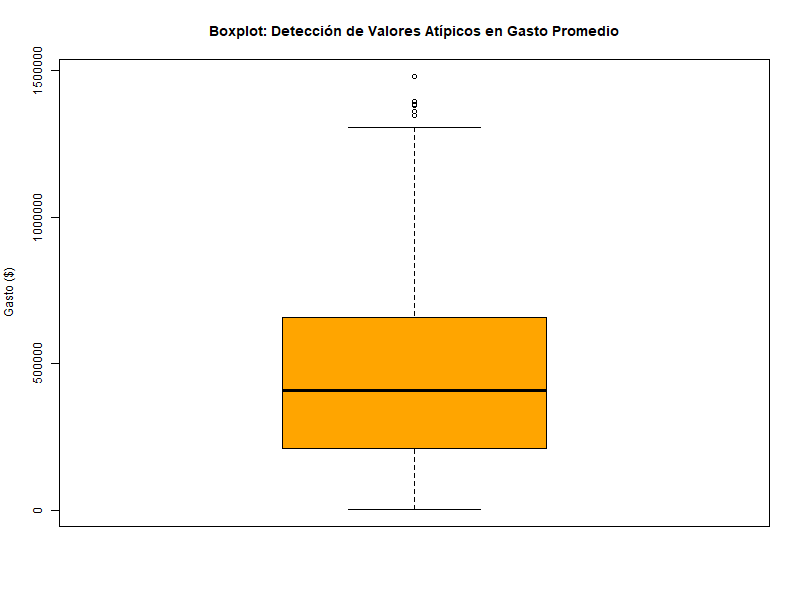
\includegraphics[width=0.8\textwidth]{grafico_outliers.png}
    \caption{Detección de valores atípicos en Gasto Promedio (Método IQR).}
    \label{fig:outliers}
\end{figure}

\textbf{Implicancias:} Estos \textbf{Clientes VIP} provienen de comunas de altos ingresos y su comportamiento es clave para el volumen de ventas. Deben ser segmentados para recibir tratamiento exclusivo (ej., atención personalizada, preventas, beneficios de lealtad elevados).

\section*{6. Clustering o segmentación (Pregunta 3)}
El análisis de segmentación se realizó mediante el algoritmo \textbf{K-Means}, utilizando \textbf{$k=4$} clusters. Las variables empleadas fueron: \texttt{Numero\_Compras}, \texttt{Promedio\_Total\_Compra}, \texttt{Ratio\_Frecuencia} y \texttt{Puntos\_Socio}. Los datos fueron previamente estandarizados con la función \texttt{scale()}.

\subsection*{6.1. Interpretación de Centroides}
Los centroides, que representan el perfil promedio de cada cluster, permiten la siguiente caracterización:

\begin{table}[H]
    \centering
    \caption{Centroides (Valores Promedio) de los 4 Clusters}
    \label{tab:centroides}
    \begin{tabular}{c c c c c}
    \toprule
    \textbf{Cluster} & \textbf{Nº Compras} & \textbf{Gasto Promedio (\$)} & \textbf{Frecuencia} & \textbf{Puntos Socio} \\
    \midrule
    1 & 292 & 386.921 & 5.13 & 2184 \\
    2 & \textbf{770} & 282.768 & 5.75 & 4522 \\
    \rowcolor{gray!20} \textbf{3 (VIP)} & 605 & \textbf{879.383} & 5.63 & 5366 \\
    4 & 314 & 365.266 & 5.56 & \textbf{8095} \\
    \bottomrule
    \end{tabular}
\end{table}

\textbf{Perfiles Identificados:}
\begin{itemize}
    \item \textbf{Cluster 3 (VIP):} Clientes de **Alto Gasto Extremo** (\$879k), con una frecuencia y número de compras altos. Es el segmento de mayor valor.
    \item \textbf{Cluster 2 (Frecuentes de Bajo Valor):} Se distingue por el \textbf{mayor número de compras} (770), pero el \textbf{menor gasto promedio} (\$282k). Oportunidad para estrategias de venta cruzada (cross-selling).
    \item \textbf{Cluster 4 (Orientados a Puntos):} Clientes que compran poco (314) pero tienen la mayor cantidad de puntos de fidelidad (\textbf{8.095}). Muy sensibles a programas de lealtad.
    \item \textbf{Cluster 1 (Compradores de Frecuencia Media):} Perfil equilibrado, con valores medios en todas las variables.
\end{itemize}

El gráfico \ref{fig:clusters} muestra la separación de estos grupos.

\begin{figure}[H]
    \centering
    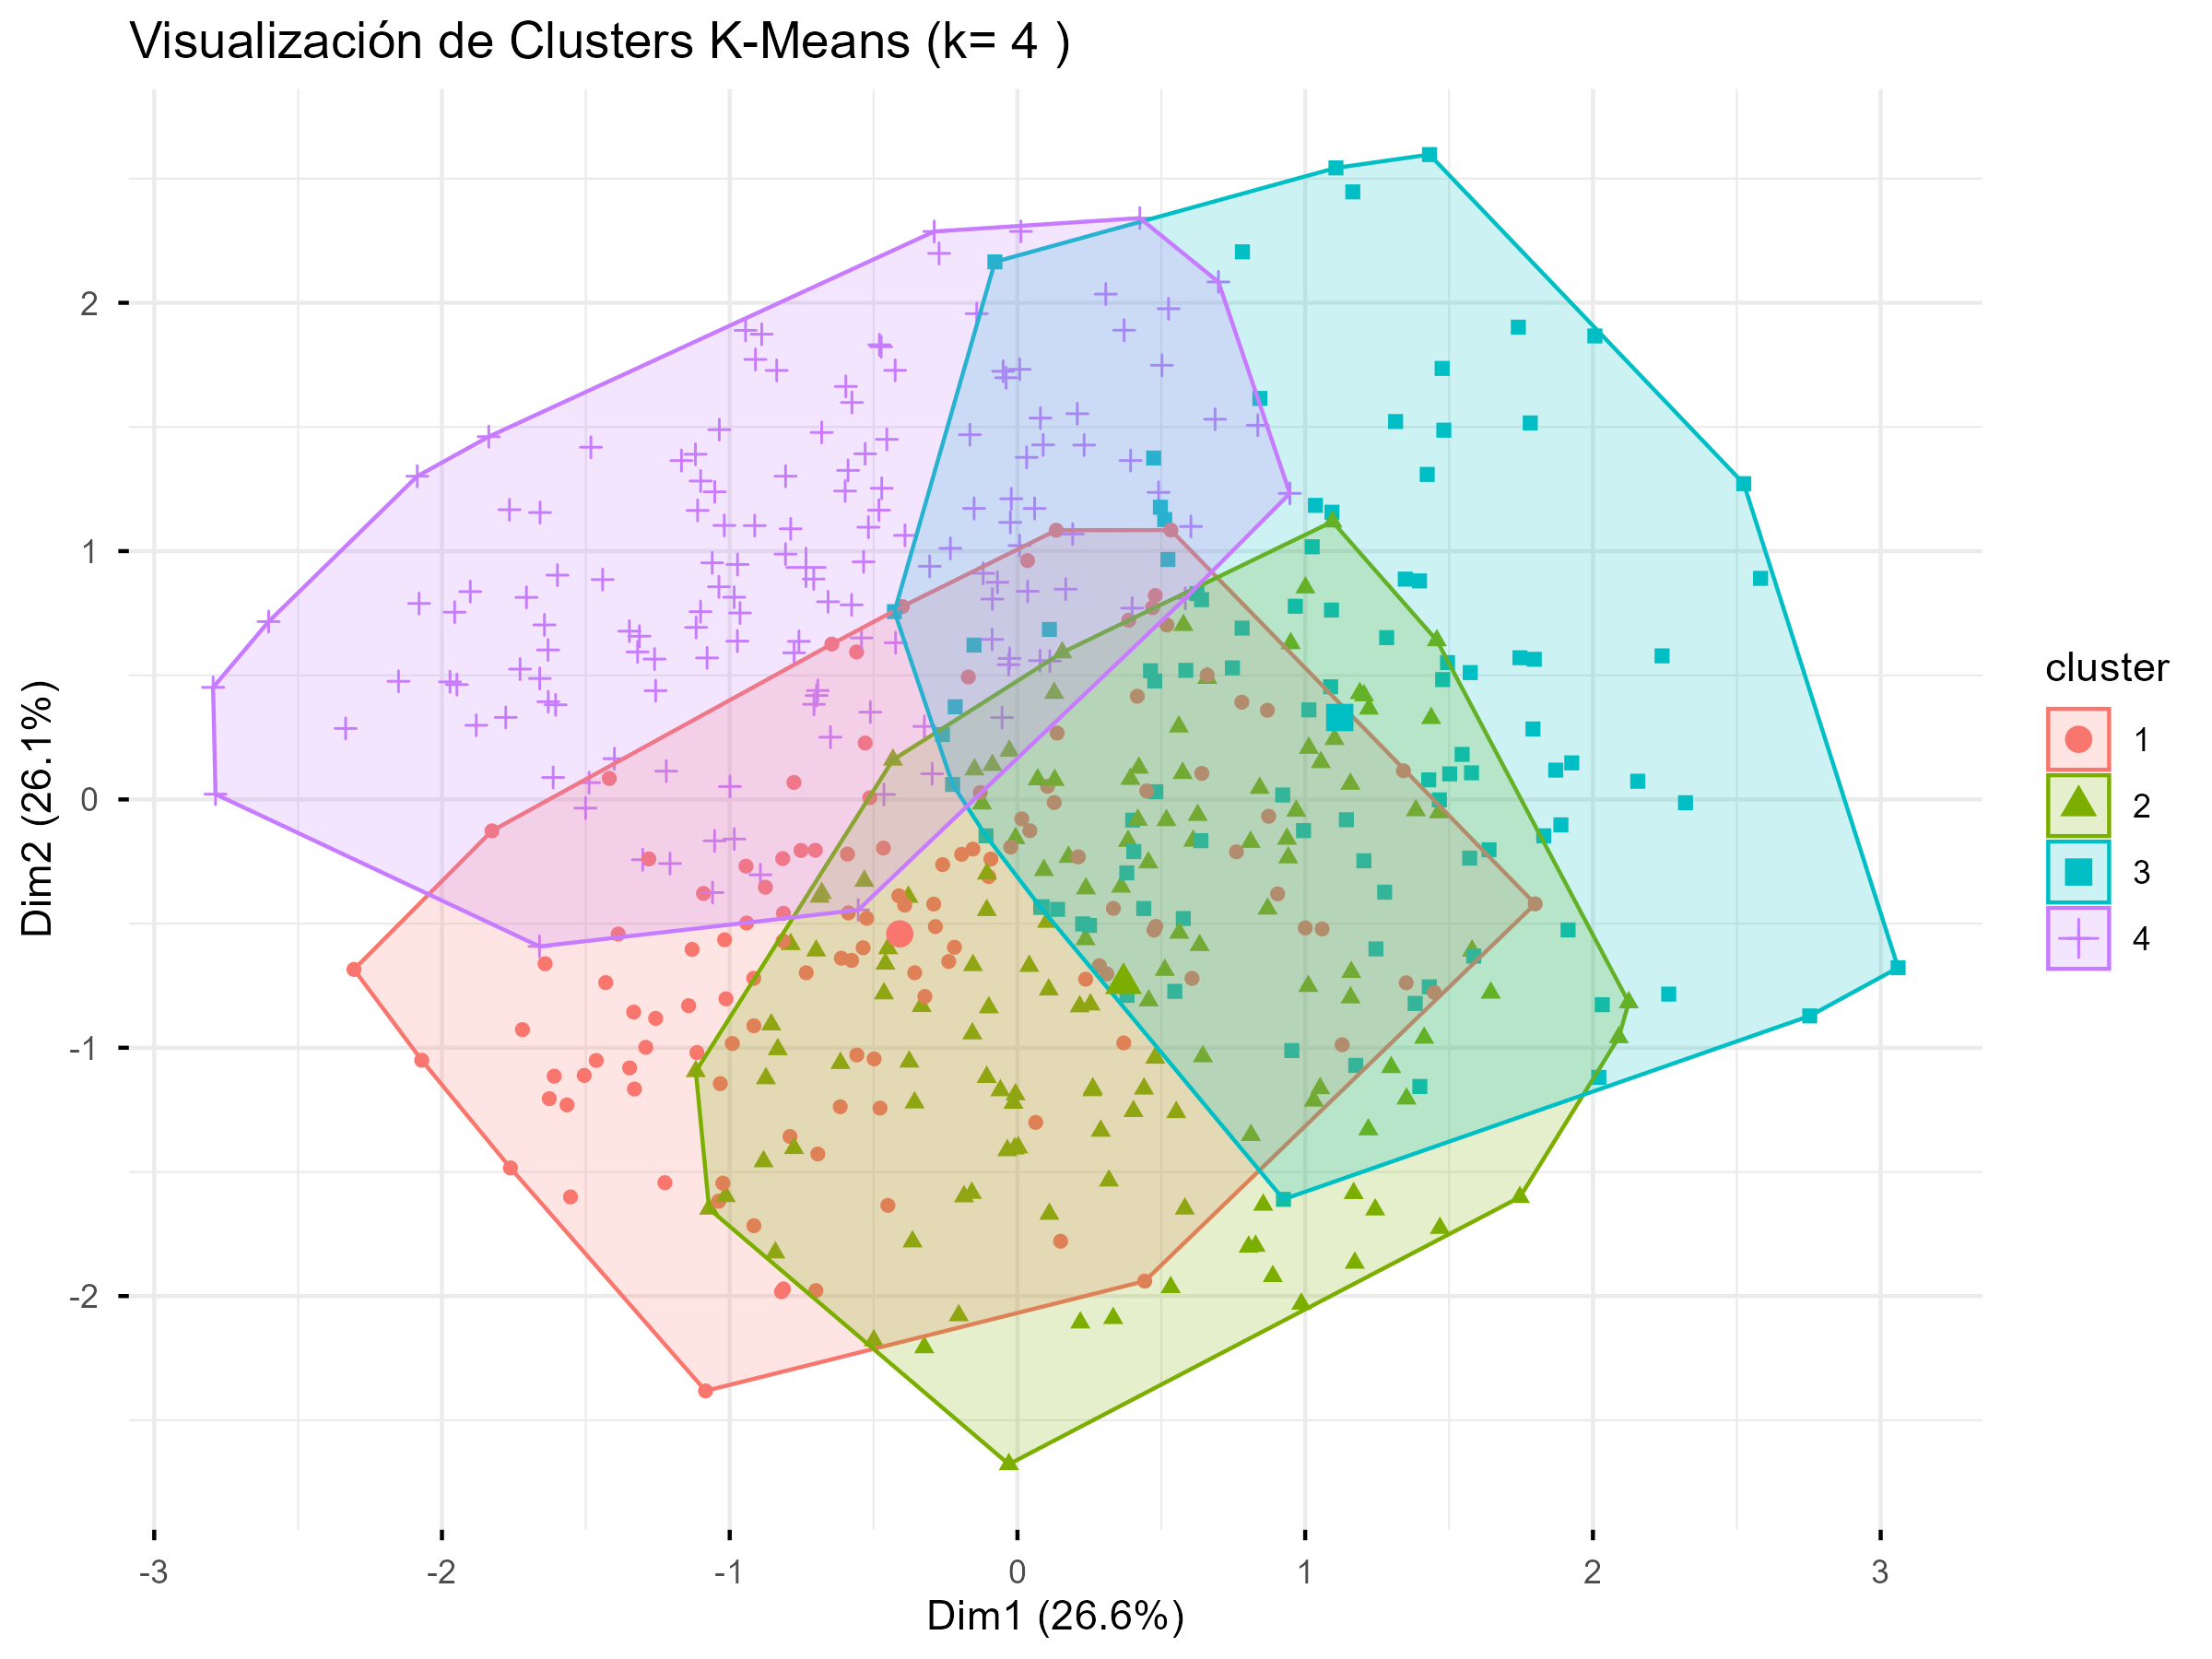
\includegraphics[width=0.8\textwidth]{grafico_clusters.png}
    \caption{Visualización de clusters K-Means.}
    \label{fig:clusters}
\end{figure}

\vspace{0.5cm}

\textbf{Ejemplo de código R utilizado para Clustering:}
\begin{verbatim}
# Escalamiento
variables_cluster <- datos_lidl %>%
  select(Numero_Compras, Promedio_Total_Compra, 
         Ratio_Frecuencia, Puntos_Socio)
datos_scaled <- scale(variables_cluster)

# Aplicación de K-Means
set.seed(42) 
k.final <- kmeans(datos_scaled, centers = 4, nstart = 25)

# Visualización
fviz_cluster(k.final, data = datos_scaled)
\end{verbatim}

\section*{7. Principales Insights y Conclusiones}
El análisis proporciona una hoja de ruta clara para la estrategia de Lidl en Chile:

\begin{itemize}
    \item \textbf{Grupos de Clientes Identificados:} Se definieron cuatro segmentos, siendo el \textbf{Cluster 3 (VIP)} el segmento de mayor valor. El \textbf{Cluster 2 (Frecuentes de Bajo Valor)} es la principal oportunidad para aumentar los ingresos por transacción.
    \item \textbf{Rentabilidad por Perfil:} Los clientes \textbf{Planificados} son los que generan el mayor gasto promedio, siendo el perfil más rentable a nivel de transacción, superando ligeramente al Entusiasta.
    \item \textbf{Variables Más Influyentes:} La variable \textbf{Promedio\_Total\_Compra} es el factor más determinante en la identificación de segmentos VIP (Cluster 3), mientras que \textbf{Numero\_Compras} define la alta actividad del Cluster 2.
    \item \textbf{Recomendaciones Estratégicas:}
    \begin{enumerate}
        \item \textbf{Fidelización VIP:} Crear un programa de lealtad de nivel "Platinum" enfocado en el Cluster 3, basado en experiencias exclusivas y no solo en descuentos.
        \item \textbf{Maximización del Gasto:} Diseñar estrategias de venta cruzada (cross-selling) dirigidas al Cluster 2 (Frecuentes de Bajo Valor) para aumentar el tamaño de su canasta promedio sin afectar su alta frecuencia.
        \item \textbf{Enfoque Geográfico:} Priorizar campañas de marketing y expansión en comunas de alto gasto promedio como Lo Barnechea, Vitacura y Providencia, donde residen los clientes de mayor valor.
    \end{enumerate}
\end{itemize}


\end{document}